\section{Methodology}
We treat each consumer-item as an individual object and generate weekly time series based on historical transaction for 
each object. The target value at each time step (week) takes a binary input, 1/0 (purchased/not purchased).
We then generate various types of features including datetime related, label encoded and target encoded 
within and across objects. Below are the feature groups with the type of features within each group:
\begin{itemize}
\item {\bf Datetime:} Transactional metrics at various temporal cuts including week, month and quarter. 
Fourier and Taylor functions to capture seasonality and trends.
\item {\bf Consumer Profile:} Total number of orders by the user, Number of distinct items ordered by the user
Time since first order by the shopper, Time since last order by the shopper, Averge time gap between orders
Reorder rate of the user, Reorder frequency of the user, Time of the day user visits, Specific item ordered by user in the past
Order size based features, Orders with no previously reordered item.
\item {\bf Item Profile:} Time since first order for the merchandise, Time since last order for the merchandise
Averge time gap between orders, Reorder rate of the item, Reorder frequency of the item
Number of co-occuring items with this item, Item's average position in the cart, Statistics around order streak for this item
Item's total number of orders, Number of distinct users, Number of users buying it as one shot item.
\item {\bf Consumer-Item Profile:} Time since first order for each combination, Time since last order for each combination
Averge time gap between orders, Reorder rate of the combination, Reorder frequency of the combination, 
Streak -user purchased the item in a row, Average position in the cart, Co-occurance Statistics
Replacement items, Total number of orders for the combination, If user already ordered the item today.
\end{itemize}
The model we needed to build, thus, should learn to identify similarly behaving time series across latent
parameters, and take into account consumer and item variations in comparing the time series. A row in time series 
is represented by

  \begin{equation}
    \begin{array}{l}
      y\textsubscript{cit}  = f(i\textsubscript{t}, c\textsubscript{t},..,c\textsubscript{t-n}, ic\textsubscript{t}
      ,..,ic\textsubscript{t-n}, d\textsubscript{t},..,d\textsubscript{t-n})
    \end{array}
    \label{eqn:fx}
  \end{equation}

where y\textsubscript{cit} is sales for consumer 'c' item ’i’ at time ’t’. 
i\textsubscript{t} is attribute of the item ’i’ like category, department, brand, color, size, etc. 
c\textsubscript{t} is attribute of the consumer 'c' like age, sex and transactional attributes. 
ic\textsubscript{t} is transactional attributes of the consumer 'c'  towards item 'i'. 
d\textsubscript{t} is derived from datetime to capture trend and seasonality. 
Finally, n is the number of time lags.

%\begin{figure}[t]
%  \centering 
%  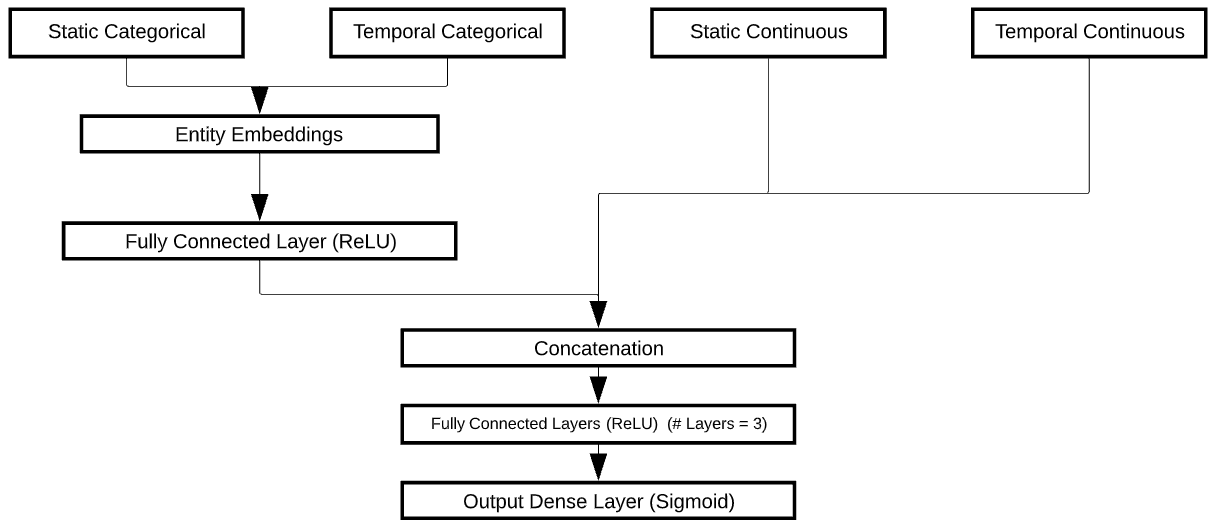
\includegraphics[width=3.3in]{img/MLP.png} 
%  \caption{Overall Approach} 
%  \label{fig:Approach} 
%\end{figure}

\subsection{Accuracy Measure}
Consumer Basket prediction framework should be able to strike good balance between Precision and Recall. 
Precision refers to the ratio of number of predicted items actually purchased from the predicted items
  \begin{equation}
      \begin{array}{l}
        Precision = \frac{TP} {TP + FP}
      \end{array}
    \label{eqn:Precision}
  \end{equation}

where TP refers to True Positive and FP refers to False Positive.
Recall refers to the ratio of predicted items actually purchased from the items in the actual basket. 
  \begin{equation}
      \begin{array}{l}
        Recall = \frac{TP} {TP + FN}
        \end{array}
    \label{eqn:Recall}
  \end{equation}

where TP refers to True Positive and FN refers to False Negative.
F1 Score is needed when you want to seek a balance between Precision and Recall.
We have previously seen that accuracy can be largely contributed by a large number of True Negatives which 
in most business circumstances, we do not focus on much whereas False Negative and False Positive usually has 
business costs, thus F1 Score might be a better measure to use if we need to seek a balance
between Precision and Recall and there is an uneven class distribution (large number of Actual Negatives).
  \begin{equation}
      \begin{array}{l}
        F1-Score = \frac{2 * Precision * Recall} {Precision + Recall}
      \end{array}
    \label{eqn:F1}
  \end{equation}

\subsection{Model Architectures}
As mentioned in previous section, traditional machine learning models are not suitable choice for solving Equation~\ref{eqn:fx}. 
Hence, we work with Deep learning models ranging from Multi-Layered Perceptron (MLP), Long Short 
Term Memory (LSTM) and Convolution Neural Network (CNN) to few of the machine learning tree based models like Random 
Forest and various flavours of Gradient Boosted Trees. Architectures of MLP, LSTM, CONV1D and CNNLSTM 
models are shown in Figure~\ref{fig:MLP}, Figure~\ref{fig:LSTM}, Figure~\ref{fig:CONV1D}
and Figure~\ref{fig:CNNLSTM}

  \begin{figure}[t]
    \centering 
    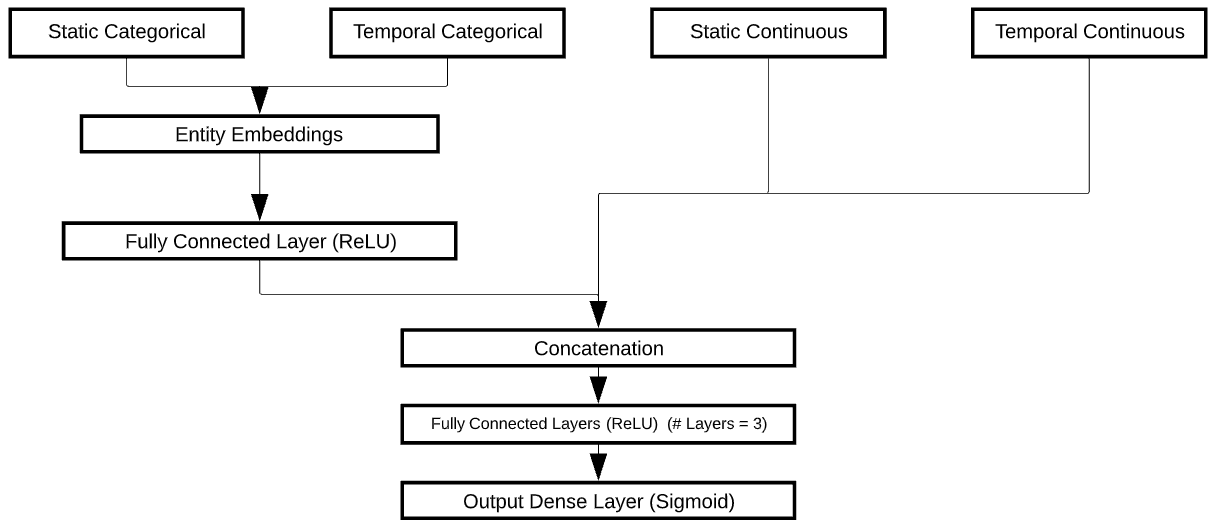
\includegraphics[width=3.3in]{img/MLP.png} 
    \caption{Multi Layer Perceptron (MLP)} 
    \label{fig:MLP} 
  \end{figure}

As mentioned in previous section, traditional machine learning models are not suitable choice for solving Equation~\ref{eqn:fx}. 
Hence, we work with Deep learning models ranging from Multi-Layered Perceptron (MLP), Long Short 
Term Memory (LSTM) and Convolution Neural Network (CNN) to few of the machine learning tree based models like Random 
Forest and various flavours of Gradient Boosted Trees. Architectures of MLP and LSTM models are shown in Figure~\ref{fig:Approach}


  \begin{figure}[t]
    \centering 
    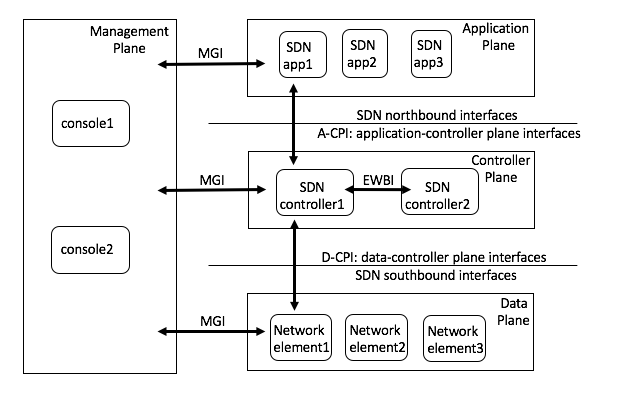
\includegraphics[width=3.3in]{img/LSTM.png} 
    \caption{Long Short Term Memory (LSTM)} 
    \label{fig:LSTM} 
  \end{figure}
As mentioned in previous section, traditional machine learning models are not suitable choice for solving Equation~\ref{eqn:fx}. 
Hence, we work with Deep learning models ranging from Multi-Layered Perceptron (MLP), Long Short 
Term Memory (LSTM) and Convolution Neural Network (CNN) to few of the machine learning tree based models like Random 
Forest and various flavours of Gradient Boosted Trees. Architectures of MLP and LSTM models are shown in Figure~\ref{fig:Approach}

  \begin{figure}[t]
    \centering 
    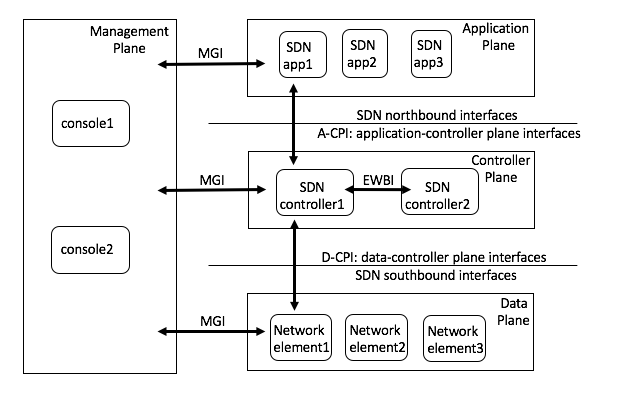
\includegraphics[width=3.3in]{img/CONV1D.png} 
    \caption{Convolution Neural Network 1D (CONV1D)} 
    \label{fig:CONV1D} 
  \end{figure}
As mentioned in previous section, traditional machine learning models are not suitable choice for solving Equation~\ref{eqn:fx}. 
Hence, we work with Deep learning models ranging from Multi-Layered Perceptron (MLP), Long Short 
Term Memory (LSTM) and Convolution Neural Network (CNN) to few of the machine learning tree based models like Random 
Forest and various flavours of Gradient Boosted Trees. Architectures of MLP and LSTM models are shown in Figure~\ref{fig:Approach}

  \begin{figure}[t]
    \centering 
    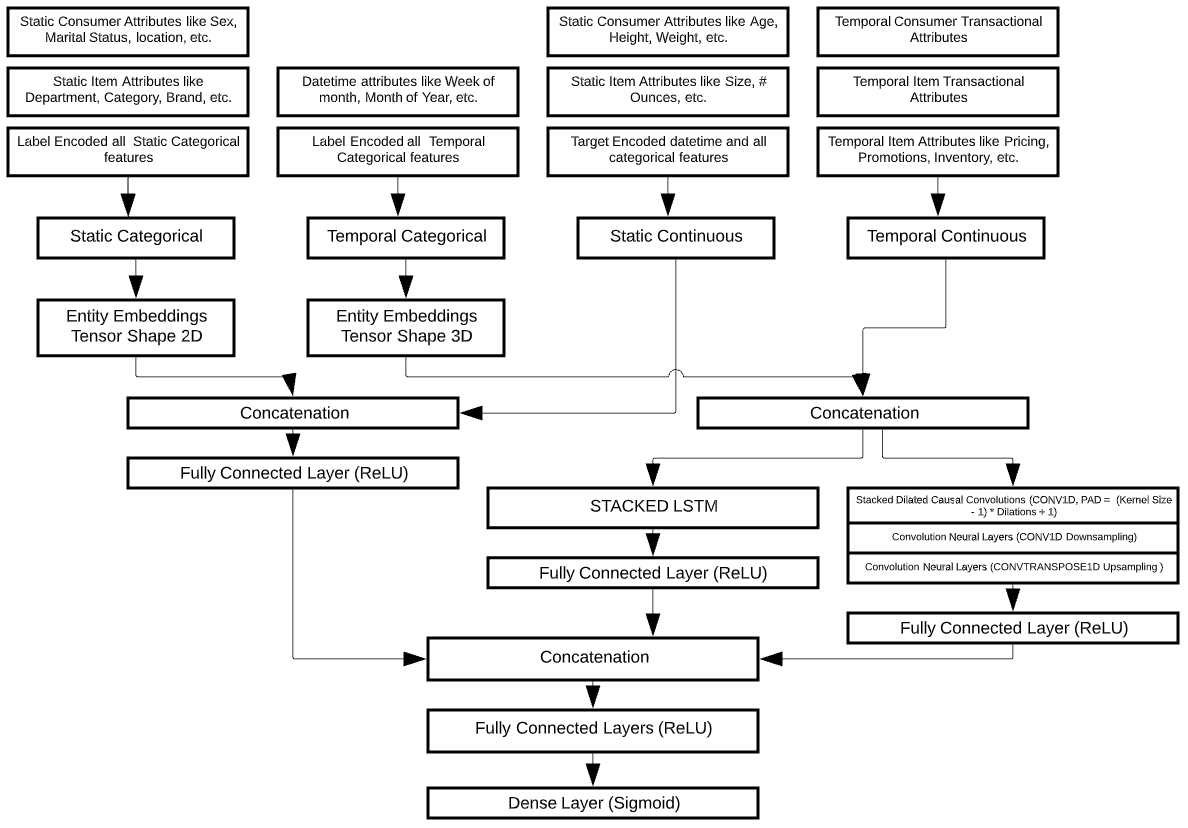
\includegraphics[width=3.3in]{img/CNNLSTM.png} 
    \caption{Convolution Neural Network 1D + Long Short Term Memory (CNNLSTM)} 
    \label{fig:CNNLSTM} 
  \end{figure}

As mentioned in previous section, traditional machine learning models are not suitable choice for solving Equation~\ref{eqn:fx}. 
Hence, we work with Deep learning models ranging from Multi-Layered Perceptron (MLP), Long Short 
Term Memory (LSTM) and Convolution Neural Network (CNN) to few of the machine learning tree based models like Random 
Forest and various flavours of Gradient Boosted Trees. Architectures of MLP and LSTM models are shown in Figure~\ref{fig:Approach}
